
	\tikzstyle{node}=[circle, draw]

	\tikzstyle{up}=[node, fill = white]
	\tikzstyle{c1}=[node, fill = white]
	\tikzstyle{md}=[node, fill = lightgray]
	\tikzstyle{c2}=[node, fill = white]
	\tikzstyle{dn}=[node, fill = white]
	\tikzstyle{ds}=[node, fill = white]
	\tikzstyle{ex}=[node, fill = white]
	\tikzstyle{nd}=[rectangle, draw]

	\begin{figure}[p]
		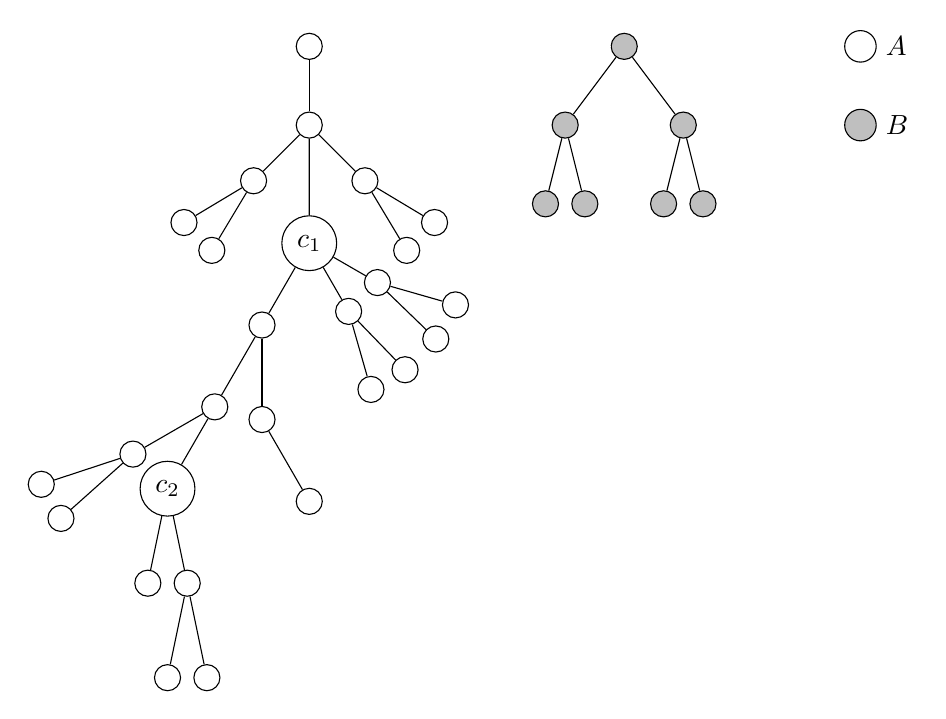
\begin{tikzpicture}
	\node[up] {}
		child[grow = south, level distance=10mm] {node[up] {}
			child[grow = south west, level distance=10mm]{node[up]{}	%left up
				[sibling distance=5mm]
				child{node[up]{}}
				child{node[up]{}}
			}
			child[level distance=15mm]{node[c1]{$c_1$} %main up
				[sibling distance=5mm]
				child [grow = -120, level distance=12mm] {node[md]{}	%1
					child[grow = -120]{node[md]{} %2
						child[grow = -150]{node[md]{}
							child{node[md]{}}
							child{node[md]{}}
						}
						child[grow = -120]{node[c2]{$c_2$} %3
							[grow = south]
							child{node[dn]{}}
							child{node[dn]{}
								child{node[dn]{}}
								child{node[dn]{}}
							}
						}
					}
					child[grow = south]{node[md]{}
						child[grow = -60]{node[md]{}}
					}
				}
				child[grow = -30, level distance=10mm]{node[ds]{}	%aux1 middle
					[sibling distance=5mm]
					child{node[ds]{}}
					child{node[ds]{}}
				}
				child [grow = -60, level distance=10mm] {node[ds]{} 	%aux2 middle
					[sibling distance=5mm]
					child{node[ds]{}}
					child{node[ds]{}}
				}
			}
			child [grow = south east, level distance=10mm] {node[up]{}	%right up
				[sibling distance=5mm]
				child{node[up]{}}
				child{node[up]{}}
			}
		}
		child[grow = east, level distance=40mm, white]{node[black, ex]{}
			[grow = south]
			[level distance=10mm]
			child[black]{node[ex]{}
				[sibling distance=5mm]
				child{node[ex]{}}
				child{node[ex]{}}
			}
			child[black] {node[ex]{}
				[sibling distance=5mm]
				child{node[ex]{}}
				child{node[ex]{}}
			}
		}
		;
		\draw [black, fill=white] (70mm,0) circle [radius=2mm];
		\node [right] at (72mm,0) {$A$};
		\draw [black, fill=lightgray] (70mm,-10mm) circle [radius=2mm]; 
		\node [right] at (72mm,-10mm) {$B$};
\end{tikzpicture}

		\caption{Proper subdivision for $(A, B) = (A^{c_1}_{c_2}, B^{c_1}_{c_2})$}
	\end{figure}
	
	\tikzstyle{up}=[node, fill = lightgray]
	\tikzstyle{c1}=[node, fill = white]
	\tikzstyle{md}=[node, fill = white]
	\tikzstyle{c2}=[node, fill = white]
	\tikzstyle{dn}=[node, fill = white]
	\tikzstyle{ds}=[node, fill = white]
	\tikzstyle{ex}=[node, fill = white]
	\tikzstyle{nd}=[rectangle, draw]

	\begin{figure}[p]
		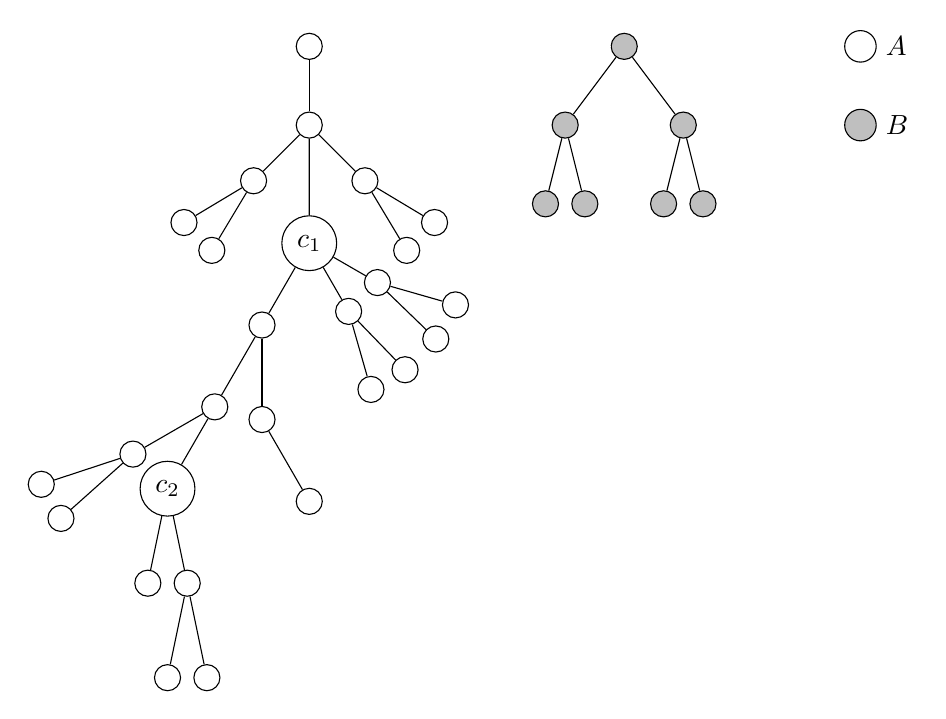
\begin{tikzpicture}
	\node[up] {}
		child[grow = south, level distance=10mm] {node[up] {}
			child[grow = south west, level distance=10mm]{node[up]{}	%left up
				[sibling distance=5mm]
				child{node[up]{}}
				child{node[up]{}}
			}
			child[level distance=15mm]{node[c1]{$c_1$} %main up
				[sibling distance=5mm]
				child [grow = -120, level distance=12mm] {node[md]{}	%1
					child[grow = -120]{node[md]{} %2
						child[grow = -150]{node[md]{}
							child{node[md]{}}
							child{node[md]{}}
						}
						child[grow = -120]{node[c2]{$c_2$} %3
							[grow = south]
							child{node[dn]{}}
							child{node[dn]{}
								child{node[dn]{}}
								child{node[dn]{}}
							}
						}
					}
					child[grow = south]{node[md]{}
						child[grow = -60]{node[md]{}}
					}
				}
				child[grow = -30, level distance=10mm]{node[ds]{}	%aux1 middle
					[sibling distance=5mm]
					child{node[ds]{}}
					child{node[ds]{}}
				}
				child [grow = -60, level distance=10mm] {node[ds]{} 	%aux2 middle
					[sibling distance=5mm]
					child{node[ds]{}}
					child{node[ds]{}}
				}
			}
			child [grow = south east, level distance=10mm] {node[up]{}	%right up
				[sibling distance=5mm]
				child{node[up]{}}
				child{node[up]{}}
			}
		}
		child[grow = east, level distance=40mm, white]{node[black, ex]{}
			[grow = south]
			[level distance=10mm]
			child[black]{node[ex]{}
				[sibling distance=5mm]
				child{node[ex]{}}
				child{node[ex]{}}
			}
			child[black] {node[ex]{}
				[sibling distance=5mm]
				child{node[ex]{}}
				child{node[ex]{}}
			}
		}
		;
		\draw [black, fill=white] (70mm,0) circle [radius=2mm];
		\node [right] at (72mm,0) {$A$};
		\draw [black, fill=lightgray] (70mm,-10mm) circle [radius=2mm]; 
		\node [right] at (72mm,-10mm) {$B$};
\end{tikzpicture}

		\caption{Proper subdivision for $(A, B) = (A_{c_1}, B_{c_1})$}
	\end{figure}

	\tikzstyle{up}=[node, fill = white]
	\tikzstyle{c1}=[node, fill = white]
	\tikzstyle{md}=[node, fill = white]
	\tikzstyle{c2}=[node, fill = white]
	\tikzstyle{dn}=[node, fill = white]
	\tikzstyle{ds}=[node, fill = lightgray]
	\tikzstyle{ex}=[node, fill = white]
	\tikzstyle{nd}=[rectangle, draw]

	\begin{figure}[p]
		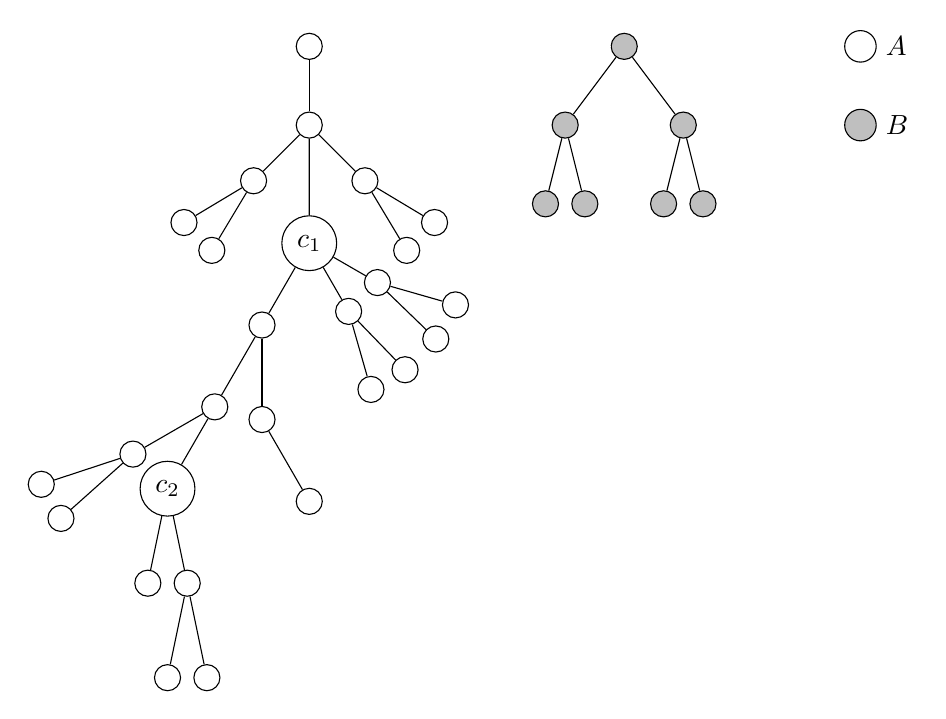
\begin{tikzpicture}
	\node[up] {}
		child[grow = south, level distance=10mm] {node[up] {}
			child[grow = south west, level distance=10mm]{node[up]{}	%left up
				[sibling distance=5mm]
				child{node[up]{}}
				child{node[up]{}}
			}
			child[level distance=15mm]{node[c1]{$c_1$} %main up
				[sibling distance=5mm]
				child [grow = -120, level distance=12mm] {node[md]{}	%1
					child[grow = -120]{node[md]{} %2
						child[grow = -150]{node[md]{}
							child{node[md]{}}
							child{node[md]{}}
						}
						child[grow = -120]{node[c2]{$c_2$} %3
							[grow = south]
							child{node[dn]{}}
							child{node[dn]{}
								child{node[dn]{}}
								child{node[dn]{}}
							}
						}
					}
					child[grow = south]{node[md]{}
						child[grow = -60]{node[md]{}}
					}
				}
				child[grow = -30, level distance=10mm]{node[ds]{}	%aux1 middle
					[sibling distance=5mm]
					child{node[ds]{}}
					child{node[ds]{}}
				}
				child [grow = -60, level distance=10mm] {node[ds]{} 	%aux2 middle
					[sibling distance=5mm]
					child{node[ds]{}}
					child{node[ds]{}}
				}
			}
			child [grow = south east, level distance=10mm] {node[up]{}	%right up
				[sibling distance=5mm]
				child{node[up]{}}
				child{node[up]{}}
			}
		}
		child[grow = east, level distance=40mm, white]{node[black, ex]{}
			[grow = south]
			[level distance=10mm]
			child[black]{node[ex]{}
				[sibling distance=5mm]
				child{node[ex]{}}
				child{node[ex]{}}
			}
			child[black] {node[ex]{}
				[sibling distance=5mm]
				child{node[ex]{}}
				child{node[ex]{}}
			}
		}
		;
		\draw [black, fill=white] (70mm,0) circle [radius=2mm];
		\node [right] at (72mm,0) {$A$};
		\draw [black, fill=lightgray] (70mm,-10mm) circle [radius=2mm]; 
		\node [right] at (72mm,-10mm) {$B$};
\end{tikzpicture}

		\caption{Proper subdivision for $(A, B) = (A^{c_1}_G, B^{c_1}_G)$ for $G = \{c_2\}$}
	\end{figure}

	\tikzstyle{up}=[node, fill = white]
	\tikzstyle{c1}=[node, fill = white]
	\tikzstyle{md}=[node, fill = white]
	\tikzstyle{c2}=[node, fill = white]
	\tikzstyle{dn}=[node, fill = white]
	\tikzstyle{ds}=[node, fill = white]
	\tikzstyle{ex}=[node, fill = lightgray]
	\tikzstyle{nd}=[rectangle, draw]

	\begin{figure}[p]
		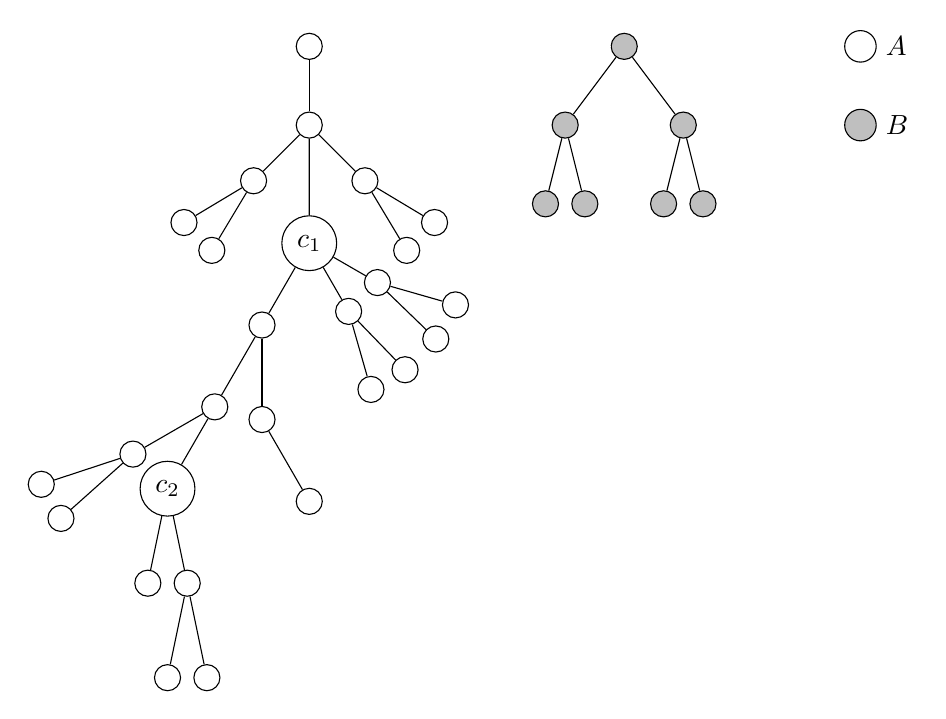
\begin{tikzpicture}
	\node[up] {}
		child[grow = south, level distance=10mm] {node[up] {}
			child[grow = south west, level distance=10mm]{node[up]{}	%left up
				[sibling distance=5mm]
				child{node[up]{}}
				child{node[up]{}}
			}
			child[level distance=15mm]{node[c1]{$c_1$} %main up
				[sibling distance=5mm]
				child [grow = -120, level distance=12mm] {node[md]{}	%1
					child[grow = -120]{node[md]{} %2
						child[grow = -150]{node[md]{}
							child{node[md]{}}
							child{node[md]{}}
						}
						child[grow = -120]{node[c2]{$c_2$} %3
							[grow = south]
							child{node[dn]{}}
							child{node[dn]{}
								child{node[dn]{}}
								child{node[dn]{}}
							}
						}
					}
					child[grow = south]{node[md]{}
						child[grow = -60]{node[md]{}}
					}
				}
				child[grow = -30, level distance=10mm]{node[ds]{}	%aux1 middle
					[sibling distance=5mm]
					child{node[ds]{}}
					child{node[ds]{}}
				}
				child [grow = -60, level distance=10mm] {node[ds]{} 	%aux2 middle
					[sibling distance=5mm]
					child{node[ds]{}}
					child{node[ds]{}}
				}
			}
			child [grow = south east, level distance=10mm] {node[up]{}	%right up
				[sibling distance=5mm]
				child{node[up]{}}
				child{node[up]{}}
			}
		}
		child[grow = east, level distance=40mm, white]{node[black, ex]{}
			[grow = south]
			[level distance=10mm]
			child[black]{node[ex]{}
				[sibling distance=5mm]
				child{node[ex]{}}
				child{node[ex]{}}
			}
			child[black] {node[ex]{}
				[sibling distance=5mm]
				child{node[ex]{}}
				child{node[ex]{}}
			}
		}
		;
		\draw [black, fill=white] (70mm,0) circle [radius=2mm];
		\node [right] at (72mm,0) {$A$};
		\draw [black, fill=lightgray] (70mm,-10mm) circle [radius=2mm]; 
		\node [right] at (72mm,-10mm) {$B$};
\end{tikzpicture}

		\caption{Proper subdivision for $(A, B) = (A_G, B_G)$ for $G = \{c_1, c_2\}$}
	\end{figure}
